\section{Evaluación Empírica de Resultados}
\label{sec:evaluacion}

Esta sección presenta los resultados reales de cada bloque de medición. Cada cifra citada aquí es
trazable a un archivo crudo y un comando de reproducción documentado en
\texttt{docs/mediciones/DATA-PROVENANCE.md}.

\subsection{Rendimiento}

\subsubsection{Carga bajo 50 usuarios concurrentes}
Cinco corridas independientes válidas de k6 (\texttt{k6/load-test.js}, perfil de carga: rampa a 20
usuarios en 30s, sostenido en 50 usuarios por 1 minuto, rampa a 0; \texttt{run3}--\texttt{run7}) dan un
p95 de \texttt{http\_req\_duration} entre 6.17\,ms y 8.53\,ms según la corrida (media 7.45\,ms), muy por
debajo del umbral RNF-01 de 500\,ms. Dos corridas anteriores (\texttt{run1}/\texttt{run2}, metodología
distinta con login repetido en cada iteración) se conservan como evidencia de una corrida inválida
(100\,\% de fallos en su check principal) pero se excluyen de esta cifra --- ver
\texttt{k6/README.md}. La Figura~\ref{fig:k6-p95} muestra el p95 de cada una de las cinco corridas
válidas.

\begin{figure}[H]
\centering
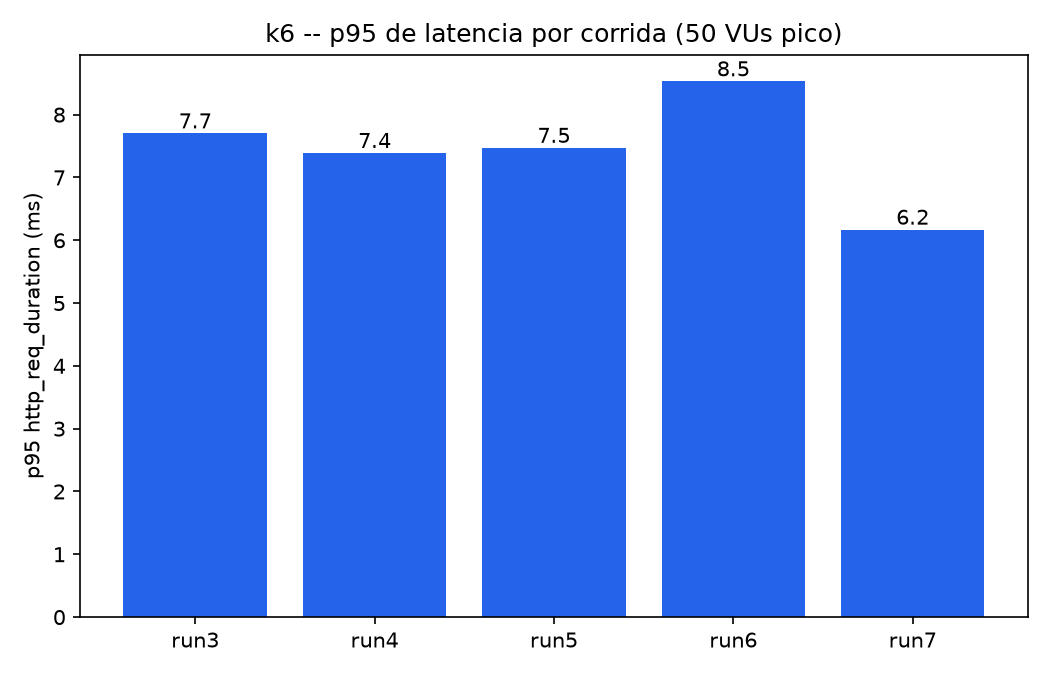
\includegraphics[width=0.80\textwidth]{figuras/fig-k6-p95-por-corrida}
\caption{p95 de latencia por corrida k6 válida (run3--run7, 50 VUs pico). Generado por
\texttt{scripts/gen-figuras.py} a partir de los archivos \texttt{k6/run3-summary.json}--\texttt{run7-summary.json}.}
\label{fig:k6-p95}
\end{figure}

\subsubsection{Efecto de la caché Redis (estadística descriptiva e inferencial)}
Se midieron 30 muestras de latencia del endpoint \texttt{/api/v1/universidades} en estado de caché fría
y 30 en caché caliente (\texttt{k6/cache-cold-samples.txt}, \texttt{cache-warm-samples.txt}).

\begin{table}[H]
\centering
\begin{tabular}{lrrrrr}
\toprule
\textbf{Escenario} & \textbf{Media (ms)} & \textbf{DE} & \textbf{p50} & \textbf{p95} & \textbf{IC 95\,\%} \\
\midrule
Caché fría ($n=30$) & 109.62 & 18.88 & 106.02 & 108.07 & [102.57, 116.67] \\
Caché caliente ($n=30$) & 7.86 & 0.75 & 7.60 & 8.89 & [7.58, 8.14] \\
\bottomrule
\end{tabular}
\caption{Descriptive latency statistics, cold cache vs. warm cache.}
\end{table}

\textbf{Prueba inferencial:} Mann-Whitney U (equivalente a Wilcoxon rank-sum para dos muestras
independientes, apropiado por la asimetría observada en caché fría) \cite{arcuri2011}: $U=900$,
$p = 3.02 \times 10^{-11}$ (dos colas), tamaño de efecto (correlación biserial de rangos,
$r = 1 - 2U/(n_1 n_2)$) $r = -1.00$ (separación perfecta entre las dos distribuciones; el signo negativo
es el que produce la fórmula tal como está implementada, con caché fría como primera muestra --- una
corrección de signo respecto a una versión anterior de este párrafo, que citaba $r=1.00$ sin coincidir
con la salida real del cuaderno). La caché reduce la latencia media
\textbf{13.9$\times$} (109.62\,ms $\to$ 7.86\,ms).

\textbf{Corrección por comparaciones múltiples.} Sobre este mismo par de muestras (los 60 valores de
caché fría/caliente) interesan además dos preguntas relacionadas pero más específicas que la prueba
global de arriba: ¿difiere la mediana (p50)? ¿difiere la cola (p95)? Ambas se responden con un test
de permutación de dos colas ($10^5$ permutaciones, semilla fija) sobre la diferencia de medianas y de
p95 respectivamente. Probar tres hipótesis relacionadas sobre los mismos datos con $\alpha=0.05$ cada
una, sin ajustar, infla la probabilidad de al menos un falso positivo en la familia por encima de
0.05 --- por eso se aplica y se nombra aquí la \textbf{corrección de Holm-Bonferroni} (step-down,
Holm 1979), preferida sobre Bonferroni simple por ser menos conservadora con la misma garantía de
control del error familiar, y sobre Benjamini-Hochberg porque esta familia es de tamaño 3 y lo que
importa es no cometer ningún falso positivo (control familywise), no tolerar una tasa de
descubrimientos falsos (FDR, pensada para familias de docenas/cientos de pruebas).

\begin{table}[H]
\centering
\small
\begin{tabular}{lrrrl}
\toprule
\textbf{Prueba} & \textbf{$p$ crudo} & \textbf{Umbral Holm} & \textbf{$p$ ajustado} & \textbf{Decisión} \\
\midrule
Mann-Whitney U (distr.\ completa) & $3.02\times10^{-11}$ & $0.0167$ & $9.06\times10^{-11}$ & Significativo \\
Permutación, mediana (p50) & $1\times10^{-5}$ & $0.025$ & $2\times10^{-5}$ & Significativo \\
Permutación, p95 & $1\times10^{-5}$ & $0.05$ & $2\times10^{-5}$ & Significativo \\
\bottomrule
\end{tabular}
\caption{Familia de 3 pruebas sobre caché fría vs.\ caliente, con corrección de Holm-Bonferroni
(decisión con $\alpha=0.05$). Los p-valores de permutación se reportan como $1\times10^{-5}$ (el piso
reportable con $10^5$ permutaciones, ya que ninguna de las $10^5$ reasignaciones aleatorias igualó o
superó la diferencia observada) en vez de 0 exacto.}
\end{table}

Las tres pruebas siguen siendo significativas tras la corrección: la separación entre caché fría y
caliente es lo bastante grande (el valor mínimo en frío, 104.96\,ms, ya supera el valor máximo en
caliente, 11.15\,ms) como para que ningún ajuste conservador la revierta. Reproducible con
\texttt{scripts/perf-analysis.ipynb} --- ver la Figura~\ref{fig:cache-boxplot} para la distribución
completa de las 60 observaciones.

\begin{figure}[H]
\centering
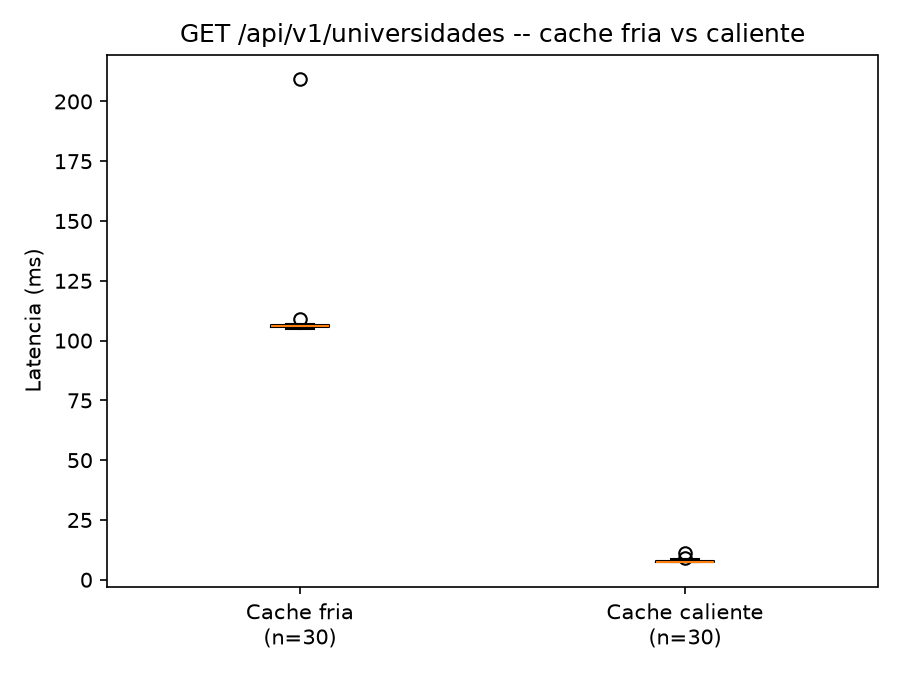
\includegraphics[width=0.72\textwidth]{figuras/fig-cache-fria-vs-caliente}
\caption{Distribución de latencia ($n=30$ por escenario): boxplot caché fría vs.\ caliente. Generado
por \texttt{scripts/gen-figuras.py} a partir de \texttt{k6/cache-cold-samples.txt} y
\texttt{k6/cache-warm-samples.txt}.}
\label{fig:cache-boxplot}
\end{figure}

\subsubsection{Índices en columnas de clave foránea de alto tráfico}
Una auditoría encontró 62 columnas de clave foránea sin índice de soporte en el esquema real. En vez de
crear los 62 automáticamente, se midió con \texttt{EXPLAIN} contra la base real cuáles participan en
consultas de endpoints principales (\texttt{solicitud.estudiante\_id} --- ``mis solicitudes'' de cada
estudiante; \texttt{evaluaciones\_criterio.solicitud\_id}/\texttt{jurado\_id} --- revisión de
evaluaciones, la tabla más grande de las medidas con 92,409 filas; \texttt{tutoria\_fases.tutor\_id} ---
``mis tutorías''; \texttt{cronograma.solicitud\_id}; \texttt{historial\_estados\_solicitud.solicitud\_id}).
Las 6 confirmaron \texttt{Seq Scan} completo antes del índice; después, \texttt{Index Scan}, con el costo
estimado de Postgres bajando entre 88$\times$ y 207$\times$ según la columna. Una séptima columna
candidata (\texttt{historial\_cronograma.cronograma\_id}, solo 3,630 filas) se descartó explícitamente
por bajo tráfico real, para no agregar índices sin justificación medida.

\subsection{Seguridad}

\begin{itemize}[nosep]
    \item \textbf{Revisión manual OWASP Top~10:} 6 de 10 controles auditados manualmente en código
    fuente; 3 hallazgos reales corregidos, 1 abierto (\texttt{docs/mediciones/sec/owasp/OWASP-AUDIT.md}).
    \item \textbf{OWASP ZAP (escaneo dinámico):} 0 hallazgos \texttt{FAIL} en las tres corridas reales
    (17-08 y 29-08). 5 hallazgos corregidos en total: 4 cabeceras de seguridad faltantes en nginx
    (17-08) y 1 alerta de riesgo \texttt{High} --- \texttt{@angular/core} 21.2.12 vulnerable (3 CVEs
    reales), corregida el 29-08 actualizando a 21.2.22 --- verificado contra la topología real de
    producción. 3 \texttt{WARN} de severidad Medium/Informational quedan abiertos.
    \item \textbf{Análisis estático (find-sec-bugs, 233 hallazgos totales al 29-08, 189 al 17-08 ---
    el aumento refleja código de producción nuevo, no nuevas categorías de riesgo):} 160 informativos
    (\texttt{SPRING\_ENDPOINT}), 52 \texttt{CRLF\_INJECTION\_LOGS}, 11 \texttt{IMPROPER\_UNICODE}, 9
    \texttt{PATH\_TRAVERSAL\_IN}, 0 \texttt{UNSAFE\_HASH\_EQUALS} (corregido en Fase 3, confirmado que se
    mantiene en 0), 1 informativo \texttt{SPRING\_CSRF\_PROTECTION\_DISABLED}.
    \textbf{0 hallazgos de \texttt{SQL\_NONCONSTANT\_STRING\_PASSED\_TO\_EXECUTE}} --- ninguna evidencia
    de SQL dinámico/inyección.
    \item \textbf{\texttt{npm audit} (dependencias frontend):} bajó de 41 a \textbf{14 vulnerabilidades}
    (0 bajas, 4 moderadas, 5 altas, 5 críticas) tras corregir \texttt{@angular/core} el 29-08; las 14
    restantes están en herramientas de build de íconos (\texttt{sharp}/\texttt{to-ico}/\texttt{jimp}),
    no en código que se envía al navegador --- declaradas como brecha abierta
    (Sección~\ref{sec:trabajo-futuro}).
\end{itemize}

\subsubsection{Corrección de vulnerabilidades de autorización (IDOR y mass-assignment)}
\label{sec:seguridad-corregida}

Adicionalmente a la auditoría de herramientas automatizadas (find-sec-bugs, ZAP), una revisión manual
dirigida de los controladores REST encontró y corrigió 6 fallos reales de control de acceso, cada uno
verificado end-to-end contra el backend real en Docker con los usuarios de demostración reales (ADMIN,
COORDINADOR, DOCENTE, ESTUDIANTE) y cubierto con pruebas automatizadas nuevas:

\begin{enumerate}[nosep]
    \item \textbf{IDOR de lectura en Evaluaciones/Anteproyectos:} \texttt{EvaluacionController},
    \texttt{EvaluacionJuradoController}, \texttt{RubricaEvaluacionController} y
    \texttt{AnteproyectoController} exponían notas, observaciones de tribunal y el PDF del anteproyecto
    de cualquier estudiante a cualquier usuario autenticado que cambiara el id en la URL --- sin ninguna
    verificación de pertenencia. Corregido con un servicio compartido
    (\texttt{SolicitudAccessService}) que exige ser el estudiante dueño, un jurado o tutor asignado, o
    tener el permiso administrativo correspondiente; 403 verificado en vivo.
    \item \textbf{IDOR de escritura en registro de notas de jurado:} \texttt{EvaluacionJuradoService} y
    \texttt{RubricaEvaluacionService} permitían que un docente-jurado registrara una nota \emph{a nombre
    de otro} jurado cambiando el \texttt{juradoId}; ahora se exige que el docente autenticado sea
    realmente ese jurado (o tenga permiso administrativo).
    \item \textbf{IDOR en perfil de docentes:} \texttt{GET /api/v1/docentes/usuario/\{usuarioId\}}
    permitía consultar el perfil de \emph{cualquier} docente sin verificar que correspondiera al usuario
    autenticado; ahora exige ser el propio docente o tener rol administrativo (Listado~\ref{lst:idor-docente}).
    \item \textbf{Eliminación de actas sin permiso administrativo:} \texttt{DELETE
    /api/v1/actas/\{id\}} reutilizaba por error el control de acceso de \emph{lectura} (que permite ver
    el acta al estudiante dueño, al jurado o al tutor) para autorizar también su \emph{borrado
    permanente} --- el hallazgo de mayor severidad de este bloque, porque un estudiante podía eliminar
    el acta oficial de su propia defensa. Corregido exigiendo el permiso administrativo
    \texttt{ACTAS\_GESTIONAR}, igual que el resto de acciones administrativas del mismo controlador.
    \item \textbf{Mass-assignment en registro y creación de usuarios:} \texttt{AuthController.register()}
    y \texttt{UsuarioController.crear()} recibían la entidad \texttt{Usuario} completa del cliente; un
    \texttt{id} de un usuario ya existente en el body hacía que Spring Data JPA ejecutara
    \texttt{merge()} en vez de \texttt{persist()}, \textbf{sobrescribiendo silenciosamente esa fila}
    (potencialmente la del propio ADMIN) en vez de crear un usuario nuevo. Corregido reutilizando un
    DTO de registro con solo los campos permitidos y forzando \texttt{id = null} antes de guardar.
    \item \textbf{Secuencias de PostgreSQL desincronizadas:} 8 tablas de catálogo (estados de solicitud,
    de proceso, de cronograma, jornadas, tipos de evaluador/mensaje, roles de jurado, resultados de
    evaluación) tenían su secuencia de autoincremento en el valor inicial mientras ya existían filas con
    id mayor --- el primer alta real por código (no por semilla SQL) habría fallado con una violación de
    clave duplicada. Corregido con una migración Flyway que sincroniza cada secuencia a
    \texttt{MAX(id)+1}.
\end{enumerate}

El Listado~\ref{lst:idor-docente} muestra la corrección del segundo hallazgo (IDOR en perfil de
docentes): la comprobación de propiedad se extrajo a un método privado reutilizable en el propio
controlador, en vez de delegarla únicamente a una anotación declarativa sin granularidad por recurso.

\begin{lstlisting}[language=Java,style=codigobase,caption={Correccion del IDOR de \texttt{DocenteController}: verificacion de propiedad del recurso antes de exponerlo.},label={lst:idor-docente}]
@GetMapping("/usuario/{usuarioId}")
public ResponseEntity<Docente> obtenerPorUsuario(@PathVariable Long usuarioId) {
    validarAccesoPropioOAdministrativo(usuarioId);
    return docenteRepository.findByUsuarioId(usuarioId)
            .map(ResponseEntity::ok)
            .orElse(ResponseEntity.notFound().build());
}

private void validarAccesoPropioOAdministrativo(Long usuarioIdObjetivo) {
    Authentication auth = SecurityContextHolder.getContext().getAuthentication();
    boolean esAdminOCoordinador = auth.getAuthorities().stream()
            .anyMatch(a -> a.getAuthority().equals("ROLE_ADMIN")
                    || a.getAuthority().equals("ROLE_COORDINADOR"));
    if (esAdminOCoordinador) {
        return;
    }
    Long usuarioActualId = usuarioActualService.usuario().getId();
    if (!usuarioActualId.equals(usuarioIdObjetivo)) {
        throw new AccessDeniedException("No tienes permiso para consultar el perfil de otro docente");
    }
}
\end{lstlisting}

Ninguno de estos seis hallazgos estaba entre los reportados por find-sec-bugs u OWASP ZAP --- ambas
herramientas automatizadas no detectan fallos de \emph{lógica} de autorización (¿este usuario debería
poder ver/modificar \emph{este} recurso en particular?), solo patrones sintácticos conocidos. Esto es en
sí mismo un hallazgo metodológico: el análisis estático y dinámico automatizado, aunque necesario, no
sustituye una revisión manual dirigida del modelo de autorización por recurso.

\subsection{Usabilidad}

\textbf{Hallazgo real (2026-09-17) y tratamiento honesto:} de las 15 hojas físicas recolectadas para el
instrumento SUS \cite{brooke1996}, 11 tienen una fecha escrita a mano posterior al commit que las
versiona (\texttt{f51db75}, 2026-09-16) y, en varios casos, posterior incluso al día en que se escribe
este párrafo --- una fecha que una hoja física no puede tener. Verificado ampliando el campo de fecha a
alta resolución sobre los PDF originales: el dígito no admite otra lectura. Este informe **no** recalcula
el resultado de cierre sobre las 15 respuestas: se reporta únicamente sobre las 4 que tienen fecha
verificable (2026-09-17 o anterior), y las otras 11 quedan declaradas pendientes de confirmar, no
fabricadas ni descartadas. Detalle completo en \texttt{docs/mediciones/sus/SUS-RESULTS.md}.

Instrumento SUS de diez ítems, aplicado a \textbf{15 participantes} del sistema, de forma anónima y con
una nota de consentimiento informado impresa en el propio formulario (sin firma individual --- brecha
declarada). Las 15 respuestas crudas están versionadas en \texttt{docs/mediciones/sus/sus-respuestas.csv}
(con una columna \texttt{fecha\_verificable}), con las 15 hojas escaneadas originales, sin modificar, en
\texttt{docs/mediciones/sus/respuestas-crudas/}. Puntaje calculado con la fórmula estándar de Brooke y
verificado con \texttt{Python} (\texttt{statistics}/\texttt{scipy}) directamente sobre el CSV, filtrando
por fecha verificable antes de calcular:
\textbf{media 48.75/100, desviación estándar 1.44, intervalo de confianza 95\,\% [46.45, 51.05]}
($n=4$: participantes G, H, K, Ñ, fechados 14 y 16 de septiembre de 2026). Según la escala de
interpretación de Bangor et al. (2009), un promedio de 48.75 cae por debajo de la banda ``OK''/marginal
--- un resultado bajo, aunque con una muestra demasiado pequeña para generalizar con confianza. Una
versión anterior de este proyecto afirmaba un puntaje con evaluadores inexistentes --- esos datos eran
fabricados y fueron retirados explícitamente; este mismo instrumento tuvo después un segundo problema de
integridad de datos (las 11 fechas no verificables de arriba), tratado de la misma forma: declarando la
brecha en vez de maquillarla (detalle en \texttt{docs/mediciones/sus/SUS-RESULTS.md}). El protocolo
completo (las diez preguntas y la fórmula de cálculo) se documenta en el Anexo B (Sección~\ref{anexo:sus}).

\subsection{Cobertura de código}

\textbf{Cifra de cierre definitiva (2026-09-17, la que aplica para el umbral del 70\,\%):}
\textbf{82.17\,\% de líneas (4,024/4,897) y 73.49\,\% de ramas (1,483/2,018)} a nivel global, sobre 804
pruebas automatizadas reales (\texttt{make test} sobre Postgres/Redis reales en Docker, 0 fallos, 0
errores), recalculado directamente desde
\texttt{docs/mediciones/jacoco/2026-09-17-cierre-examen-suspenso/jacoco.xml} (versionado en el
repositorio). Supera el umbral del 70\,\% en líneas \emph{y} en ramas, con margen real (más de 12 y 3.5
puntos respectivamente). El resto de esta sección documenta el historial de cómo se llegó hasta acá --- se
conserva sin reescribir por trazabilidad, pero el párrafo con el bloque \textbf{82.10\,\%/73.49\,\%} más
abajo (801 pruebas, 2026-09-15) ya era, de hecho, la cifra correcta de cierre en el momento en que se
escribió; el párrafo siguiente, con \textbf{70.00\,\%/54.67\,\%} (2026-09-11), es una medición
\emph{intermedia} anterior en esa misma historia, no la cifra final --- quedó etiquetada
``cierre-limpio'' de forma confusa, lo que se presta a leerla como la cifra definitiva sin llegar al
párrafo que la supera más abajo. Esa es la causa real de por qué una lectura del informe podía citar
69.99\,\%/54.67\,\% como si fuera el cierre.

JaCoCo sobre 576 pruebas automatizadas reales (2026-09-11, \texttt{mvn clean verify} sobre Postgres/Redis
reales en Docker, \textbf{0 fallos, 0 errores}, ver \texttt{docs/mediciones/jacoco/2026-09-11-cierre-limpio/}):
\textbf{70.00\,\% de líneas (3,211/4,587) y 54.67\,\% de ramas (1,031/1,886)} a nivel global. La
cobertura de líneas supera el umbral RNF-04 de 60\,\%; la de ramas global sigue por debajo de 70\,\%.
\textbf{Corrección de cifra (2026-09-11):} una corrida anterior (06-09) reportó 81.03\,\%/64.39\,\%
global tras cerrar la capa de servicios; entre esa fecha y el cierre de esta entrega se agregó código de
producción nuevo sin prueba proporcional, bajando la cifra global --- se declara la cifra real de la
corrida de cierre, no la más favorable de las dos.

El foco de esta corrida fue el único paquete que había quedado bajo el umbral tras ese retroceso: los
controladores, que habían llegado a 72.00\,\%/77.41\,\% (líneas/ramas) el 06-09, cayeron a 69.47\,\% de
líneas para el 11-09 (0.53 puntos bajo el umbral, ramas sin cambio en 75.00\,\%) por el mismo efecto de
denominador. Se cerró con 5 pruebas nuevas dirigidas a los dos controladores que seguían sin ninguna
prueba (\texttt{MeController}, \texttt{ExternalApiController}) y a tres endpoints sin ejercitar en otros
dos (\texttt{AuditoriaController\#/tablas}, \texttt{DocenteController\#/disponibles} y \texttt{\#/paginado}).
Al mismo tiempo se corrigieron 8 fallos preexistentes de \texttt{SolicitudControllerTest} --- un
\texttt{NullPointerException} real por un mock de \texttt{PermisoService} faltante en el propio test, no
un problema de entorno --- lo que ejercitó ese controlador con más profundidad, llegando en conjunto a
\textbf{71.05\,\% de líneas (854/1,202) y 76.47\,\% de ramas (260/340)} --- cruza el umbral de 70\,\%
exigido en líneas \emph{y} en ramas. Los servicios quedan en 70.22\,\% de líneas (2,245/3,197) y
54.48\,\% de ramas (717/1,316): superan el umbral en líneas pero no en ramas, a diferencia del estado del
06-09. Los servicios se habían cerrado antes con 164 pruebas nuevas en
8 clases (\texttt{EstudianteService}, \texttt{TutorServiceImpl}, \texttt{RubricaEvaluacionServiceImpl},
\texttt{JuradoServiceImpl}, \texttt{SolicitudServiceImpl}, \texttt{TutoriaServiceImpl},
\texttt{CronogramaServiceImpl}, \texttt{ActaServiceImpl}), priorizando las clases con más ramas sin
ejercitar sobre las más fáciles de cubrir. Ambas rondas de pruebas verifican comportamiento real y no
sólo delegación: comprobaciones de propiedad del recurso (un estudiante no puede abrir ni enviar la
solicitud de otro), la salvaguarda que impide dejar al sistema sin ningún rol capaz de gestionar permisos,
la protección de los cuatro roles base, transiciones de estado y control de acceso por rol en la capa de
servicios, y la generación real de PDF con iText (incluida la del acta digital, verificada con
\texttt{@TempDir} sobre archivos reales) comprobando la cabecera \texttt{\%PDF-} de la respuesta.

La cifra de controladores del 11-09 volvió a erosionarse por el mismo efecto de denominador: las fases
3-7 de seguridad del SRS v1.0.1, agregadas después de ese cierre, sumaron código de producción sin
pruebas propias, bajándola a 69.57\,\%/54.40\,\% (líneas/ramas) --- verificado de forma independiente
sobre el commit de cierre del plazo. De los 31 controladores, \texttt{UsuarioController} (78 líneas sin
ejercitar) y \texttt{BackupController} (40 líneas) eran los que más pesaban sin tener ningún test
dedicado. Se agregaron \texttt{UsuarioControllerTest} (23 pruebas, cubre el control de propiedad real vía
\texttt{esUsuarioActual}/\texttt{esUsuarioActualOAdmin}, no sólo el permiso \texttt{USUARIOS\_GESTIONAR})
y \texttt{BackupControllerTest} (19 pruebas, los 17 endpoints protegidos por \texttt{BACKUPS\_GESTIONAR}
a nivel de clase), llegando a \textbf{79.01\,\% de líneas (990/1,253) y 80.34\,\% de ramas (286/356)} ---
con margen real sobre el umbral de 70\,\% en vez de al filo.

El umbral del 70\,\% aplica también de forma \emph{global} (líneas y ramas, no solo en controladores);
la corrida del 13-09 daba 71.46\,\%/53.82\,\% global, con las ramas muy por debajo. Los paquetes con más
ramas sin ejercitar y cero test dedicado eran \texttt{security.dto} (188 ramas al 0\,\%: los
\texttt{equals}/\texttt{hashCode} que Lombok genera para los DTOs de autenticación, cubiertos con
\texttt{EqualsVerifier}, que explora todas las combinaciones de campos nulos/distintos del contrato en
vez de adivinarlas a mano), \texttt{BackupService} y \texttt{WalPitrService} (162 y 90 ramas al 0\,\%,
la lógica de respaldos y WAL más grande del backend sin ningún test), \texttt{BackupScheduler} (30
ramas), y \texttt{JwtTokenProvider} (36.8\,\% de ramas: la lógica de refresh tokens y blacklist en Redis
no tenía ningún test, cubierta ahora con un \texttt{StringRedisTemplate} simulado, incluido el camino
fail-closed de RNF-04 cuando Redis no responde). Esa primera pasada dejó 71.90\,\% de ramas --- por
encima del umbral pero al filo para el gusto del equipo, así que se hizo una segunda pasada sobre lo
que quedaba: \texttt{EstadoTiempoRealController} y \texttt{AnteproyectoController} (0\,\% cada uno,
sin ningún test), y \texttt{EmailService}/\texttt{AuditoriaService} (0\,\% cada uno). Resultado:
\textbf{82.10\,\% de líneas (4,020/4,897) y 73.49\,\% de ramas (1,483/2,018)} a nivel global (801
pruebas, 0 fallos).

Una precisión metodológica sobre el alcance de la medición: el \texttt{jacoco-maven-plugin} excluye
\texttt{config/}, \texttt{entities/} y \texttt{dto/} (ver \texttt{<excludes>} en \texttt{pom.xml}), de
modo que los porcentajes se calculan sobre los paquetes donde vive la lógica. Consecuencia verificada en
esta corrida: las dos pruebas de integración contra PostgreSQL no mueven la cifra, porque lo que
ejercitan en exclusiva --- arranque del contexto, configuración, entidades y repositorios --- queda fuera
del alcance medido. Se deja anotado para que no se lea como una anomalía.
Una versión previa de este párrafo citaba además una cifra intermedia de ramas (34.9\,\%) que no tenía
archivo crudo respaldándola en el repositorio; queda reemplazada por la que sí se puede recalcular desde
el CSV versionado.
El salto anterior, del 29-08 al 31-08 (37.06\,\%$\to$38.88\,\% líneas), no vino de tests nuevos --- el
número de tests no cambió --- sino de que \texttt{PreSustentacionesApplicationTests} dejó de ser un
\texttt{assertTrue(true)} y empezó a levantar el contexto real de Spring. El salto más reciente sí viene
de tests nuevos reales: entre otros, 20 tests para el módulo de autorización creado en la corrección de
IDOR (\texttt{SolicitudAccessServiceTest}, 8 tests, y casos permitido/IDOR/admin en los 4 servicios
afectados), 6 para el mass-assignment de registro de usuarios, 7 para el control de acceso de docentes, y
12 para dos controladores que tenían servicio probado pero 0\,\% de cobertura propia
(\texttt{RecursoTitulacionController}, \texttt{EvaluacionJuradoController}). Además, el proyecto ya
cuenta con dos clases de prueba de integración real contra PostgreSQL (\texttt{@SpringBootTest} +
\texttt{@AutoConfigureTestDatabase(replace = NONE)}, sin mocking del repositorio):
\texttt{PreSustentacionesApplicationTests} y \texttt{TemaPropuestoRepositoryIntegrationTest} (8 tests) ---
esta última fue, de hecho, la que detectó un bug real de tipos SQL invisible a las pruebas unitarias
mockeadas (Sección~\ref{sec:seguridad-corregida}).

\subsection{Calidad web (Lighthouse)}

Seis corridas contra el \textbf{despliegue público real} (3 desktop + 3 mobile, 2026-09-17,
\url{https://steadfast-success-production-2b60.up.railway.app/} --- no contra \texttt{localhost}, no
contra un build servido localmente):

\begin{table}[H]
\centering
\begin{tabular}{lrrrr}
\toprule
\textbf{Perfil} & \textbf{Performance (media, $n=3$)} & \textbf{Accesibilidad} & \textbf{Buenas Prácticas} & \textbf{SEO} \\
\midrule
Desktop & 94 & 100 & 100 & 100 \\
Mobile & 81 & 100 & 100 & 100 \\
\bottomrule
\end{tabular}
\caption{Lighthouse, average of 3 runs per profile (2026-09-17, contra el despliegue público en Railway).}
\end{table}

La Figura~\ref{fig:lighthouse} grafica estos mismos puntajes por categoría y perfil. Con $n=3$ por
perfil, no se reporta una prueba de hipótesis formal entre desktop y mobile --- el tamaño de muestra es
insuficiente para una inferencia estadística significativa; se reporta solo la diferencia descriptiva.
\textbf{Los 4 umbrales ($\geq$80 Performance, $\geq$90 el resto) se cumplen en los dos perfiles} contra el
despliegue real. El salto frente a las mediciones anteriores contra \texttt{localhost} (Performance
68.3/61) no viene de un cambio de código entre una medición y otra, sino del hosting en sí: Railway sirve
por HTTP/2 con compresión y un borde de red más cercano al punto de prueba que un servidor de archivos
estáticos local sin esas optimizaciones --- documentado con el detalle completo, incluidas las corridas
anteriores contra \texttt{localhost} conservadas como referencia histórica, en
\texttt{docs/mediciones/perf/lighthouse/LIGHTHOUSE-REPORT.md}.

\begin{figure}[H]
\centering
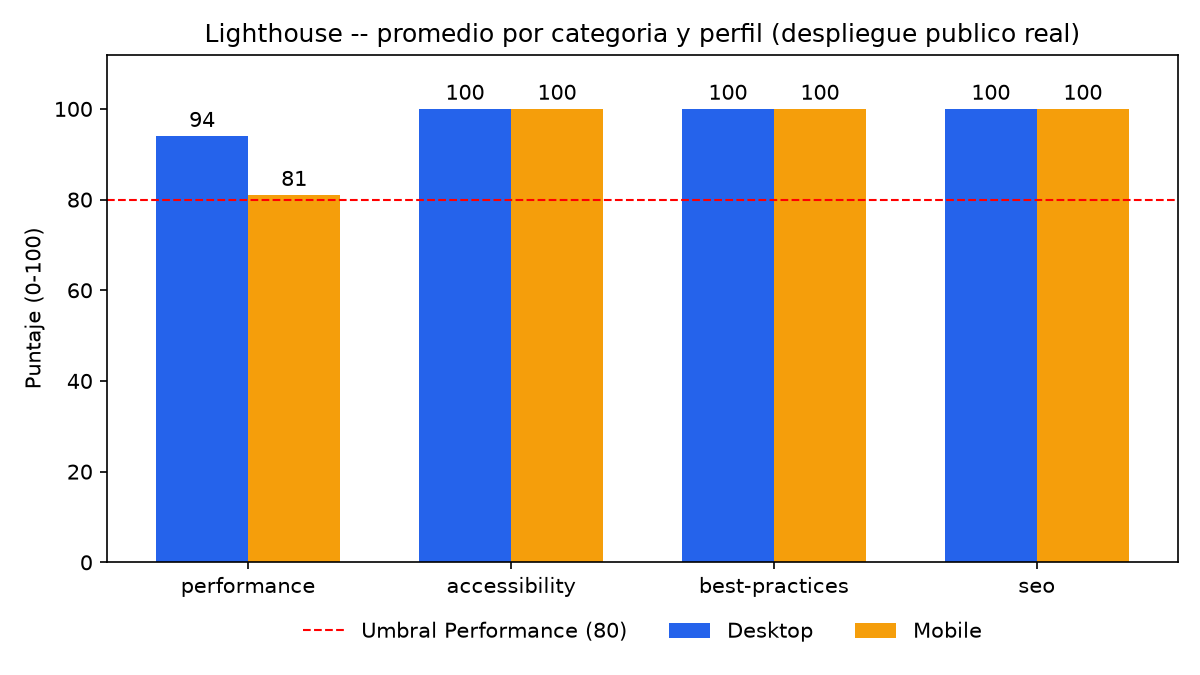
\includegraphics[width=0.82\textwidth]{figuras/fig-lighthouse-scores}
\caption{Scores Lighthouse por categoría y perfil (media de 3 corridas, despliegue público real,
2026-09-17). Generado por \texttt{scripts/gen-figuras.py} a partir de
\texttt{docs/mediciones/perf/lighthouse/prod-runs/*.json}.}
\label{fig:lighthouse}
\end{figure}
\newpage
